\documentclass{project}

\begin{document}
\title{Data logger for sensors placed in arctic conditions}
\subtitle{[Special Course - Preparatory report for fieldwork]}

%
% You need the command \numberofauthors to handle the 'placement
% and alignment' of the authors beneath the title.
%
% For aesthetic reasons, we recommend 'three authors at a time'
% i.e. three 'name/affiliation blocks' be placed beneath the title.
%
% NOTE: You are NOT restricted in how many 'rows' of
% "name/affiliations" may appear. We just ask that you restrict
% the number of 'columns' to three.
%
% Because of the available 'opening page real-estate'
% we ask you to refrain from putting more than six authors
% (two rows with three columns) beneath the article title.
% More than six makes the first-page appear very cluttered indeed.
%
% Use the \alignauthor commands to handle the names
% and affiliations for an 'aesthetic maximum' of six authors.
% Add names, affiliations, addresses for
% the se	venth etc. author(s) as the argument for the
% \additionalauthors command.
% These 'additional authors' will be output/set for you
% without further effort on your part as the last section in
% the body of your article BEFORE References or any Appendices.

\numberofauthors{1} %  in this sample file, there are a *total*
% of EIGHT authors. SIX appear on the 'first-page' (for formatting
% reasons) and the remaining two appear in the \additionalauthors section.
%
\author{
% You can go ahead and credit any number of authors here,
% e.g. one 'row of three' or two rows (consisting of one row of three
% and a second row of one, two or three).
%
% The command \alignauthor (no curly braces needed) should
% precede each author name, affiliation/snail-mail address and
% e-mail address. Additionally, tag each line of
% affiliation/address with \affaddr, and tag the
% e-mail address with \email.
%
% 1st. author
\alignauthor
Attila Sukosd\\
       \affaddr{s070600, Diplom IT, 7. semester}\\
       \email{s070600@student.dtu.dk}
}
% There's nothing stopping you putting the seventh, eighth, etc.
% author on the opening page (as the 'third row') but we ask,
% for aesthetic reasons that you place these 'additional authors'
% in the \additional authors block, viz.
\date{31 May 2011}
% Just remember to make sure that the TOTAL number of authors
% is the number that will appear on the first page PLUS the
% number that will appear in the \additionalauthors section.

\maketitle

\section{About the project}
This project is a 10 ETCS points special course, done as a collaboration between IMM and ARTEK at DTU. During the special course, an introductory course to arctic technology (course 11427) is also taken as a prerequisite for the field work in August. 

The special course runs from the 1st of March to the 26th of August, including the field work from the 28th of July to the 11th of August. 
In the first part of the project leading up to the field work, a solution will be proposed, implemented and tested. 
During the field work, the data logger will be assembled together with all the sensors, and also tested in-field.

Finally a report will be handed in after the field work to provide a detailed technical documentation as well as an evaluation of the overall project.

The supervisors are Edward Alexandru Todirica from IMM and Arne Villumsen from ARTEK. 

\section{Introduction}
\subsection{Problem Formulation}
Data collection is one of the most critical phases of any research project. Without the data, the proposed hypothesis can not be verified, thus resulting in a speculation without scientific proof of validity. 

The most basic process of data collection is based on acquiring data from different measuring devices (sensors) collect various information, save them to a file or a database to be analyzed later. There are several variables which define how "useful" is a dataset, such as the sampling rate, the resolution of the measurements and the possible error sources. In case measurements which can take months to years, the amount of continuous data collected could be a lot, and also too detailed if only a "big picture" is needed. To solve this, the measurements can be scheduled to occur at every preset interval (for example every 10 minutes), which decreases the amount of data to a more managable size, yet still provides an adequate dataset for time lapsed measurements.

Before todays' technology, where computers can be found in all shapes and forms, and connectivity is available in most parts of the world, the data collection process occured manually, by having people sit by the sensors and take measurements, however had several flaws. The accuracy of the measurements both in sampling and in resolution were dependent on the sophistication of the equipment as well as the human taking the measurements, and it was also very expensive in work-hours to have people sit by a sensor and measure it every 10 minutes for a year.

However, all of this has changed with the revolution of computers, when smaller and more powerful components are produced on a daily basis for a fraction of the price. This boom of electronics has resulted in computers being implemented in all sorts of products from household appliances to transportation and so on. Of course, there is also a solution for the data collection issues, which is nowadays called a data logger.

The data logger is an electronic device, which records the measurements from specific sensors over time and optionally sends the collected data over a (wireless) network to a central server for "live" processing. They are generally small, battery powered, portable and equipped with a microprocessor and an internal memory for storage. 

The purpose of this project is to build a general purpose data logger, which can be configured to work with a multitude of sensors, and also suitable for the arctic conditions.

\subsection{Challanges}

Since the data logger will be used in conjunction with an unattended weather station, there are several factors to consider:

\begin{itemize}\addtolength{\itemsep}{-0.5\baselineskip}
\item Sampling rate, data resolution, sources of errors
\item Power efficiency (for battery life)
\item Stability
\item Simplicity
\item Extreme conditions
\end{itemize}

As it was mentioned in the earlier section, the sampling rate, data resolution and error sources are a major consideration in choosing a suitable solution for data acquisition. Many of the data loggers on the market are only doing 1Hz sampling rate, which is not sufficient for an anenometer which can produce signals up to 125Hz depending on the wind speed. The resolution of the measurements depend on the underlying hardware, which in a data logger comes down to the resolution of the analog to digital converter (ADC) and the sources of error can be from several types of errors (such as quantization, non-linearity and apperture errors) in the ADC, as well as noise from other components and inaccuracy due to temperature fluctuations.

An other consideration when designing a system for remote locations without access to the power grid is the means to power the data logger. Battery power is an obvious choice, but the battery life of the product highly depends on the chosen components as well as the efficiency of the software for power saving. 

Stability is one of the most important challanges in creating a product which should function in a remote area for extended periods without any human intervention. This means that it should be able to recover from power failures with no data loss or damage to the device.

Since the purpose of the project is to make a general data logger, which can be reapplied in multiple senarios, it needs to be simple to set up without needing to go deep into how everything works. This can be made possible by providing an intuitive configuration with displays/buttons or easy to understand configuration files. It also means that new sensors can be added and removed without having to reprogram the microcontroller.

Finally, in the artic the environmental conditions for a data loggers are much more harsh, as there are temperature fluctuations, wind, rain, snow and ice. The effect of these could also be felt on the battery life, accuracy of measurements as well as cause hardware failures if the device is not protected sufficiently.

\subsection{Possible solutions}
ARTEK has been using data loggers for a while now, and the most popular choice was the NRG Systems SymphoniePLUS logger (\$1.395 USD) with some Symphonie SCM Cards (\$39 USD each) for the different sensors, and costs even more when communication modules are also added. (See Figure \ref{NRG})
 
\begin{figure}[!ht]
\centering
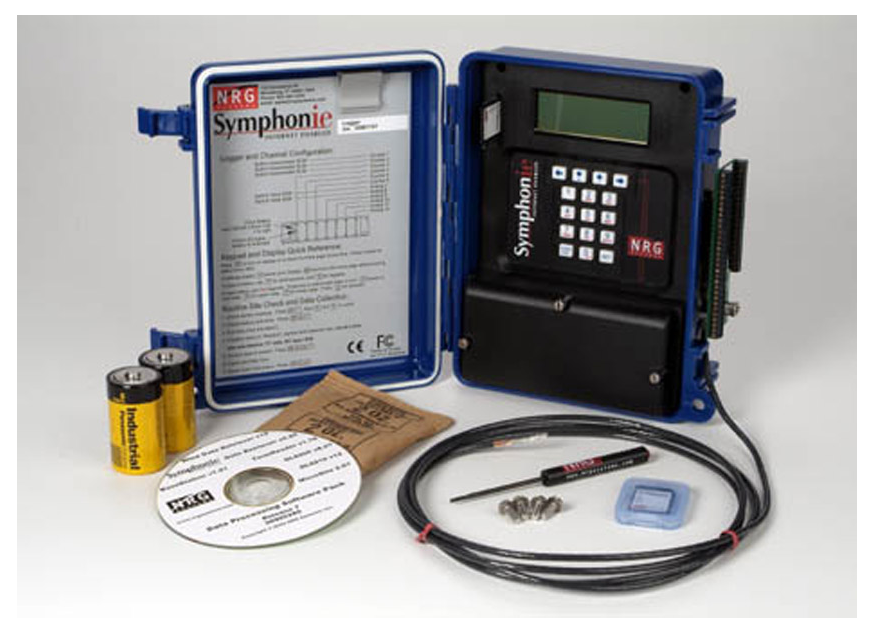
\epsfig{file=figures/NRG.eps, scale=0.4}
\caption{NRG Systems - SymphoniePLUS}
\label{NRG}
\end{figure}

After looking around the market for different kinds of data loggers, the target price of the logger per piece was set to \$300 USD, which is about 5 times cheaper than an NRG logger, while the functionality remains the same or more.

There were two different directions that were considered, microcontrollers and FPGAs. While FPGAs deliver a constant, predictable performance, microcontrollers exist in a smaller form factor with lower power consumption. For this reason, microcontrollers were chosen as the direction to go with.

From microcontrollers, there are two popular choices, the Atmel AVRs and the Microchip PIC. Both of them match roughly in all fields, including data interfaces, speed, power consumption and so on. After investigating the IDE flexibility and ease of use, an Arduino was chosen.

Arduino is an open source boot loader, board design and IDE based on the Atmel AVR chip. It provides an easy to use interface which allows the use of libraries, simplifying the development without having to rewrite a lot of code. It also register level programming, which can be used to implement new functionality or optimize the code further by hand.

Extending the hardware with further devices is also easy, as Arduinos provide a standard pinout for "shields" to use. These shields can be plugged straight on to the hardware without soldering. Most of the pins from the microcontroller are accessible through these shields, but since some pins are used up by different shields, the schematics of these have to be studied carefully to make sure they do not collide.

\section{Overview of the system}

After establishing the basic components in the system, an overview is needed.
\begin{figure}[!ht]
\centering
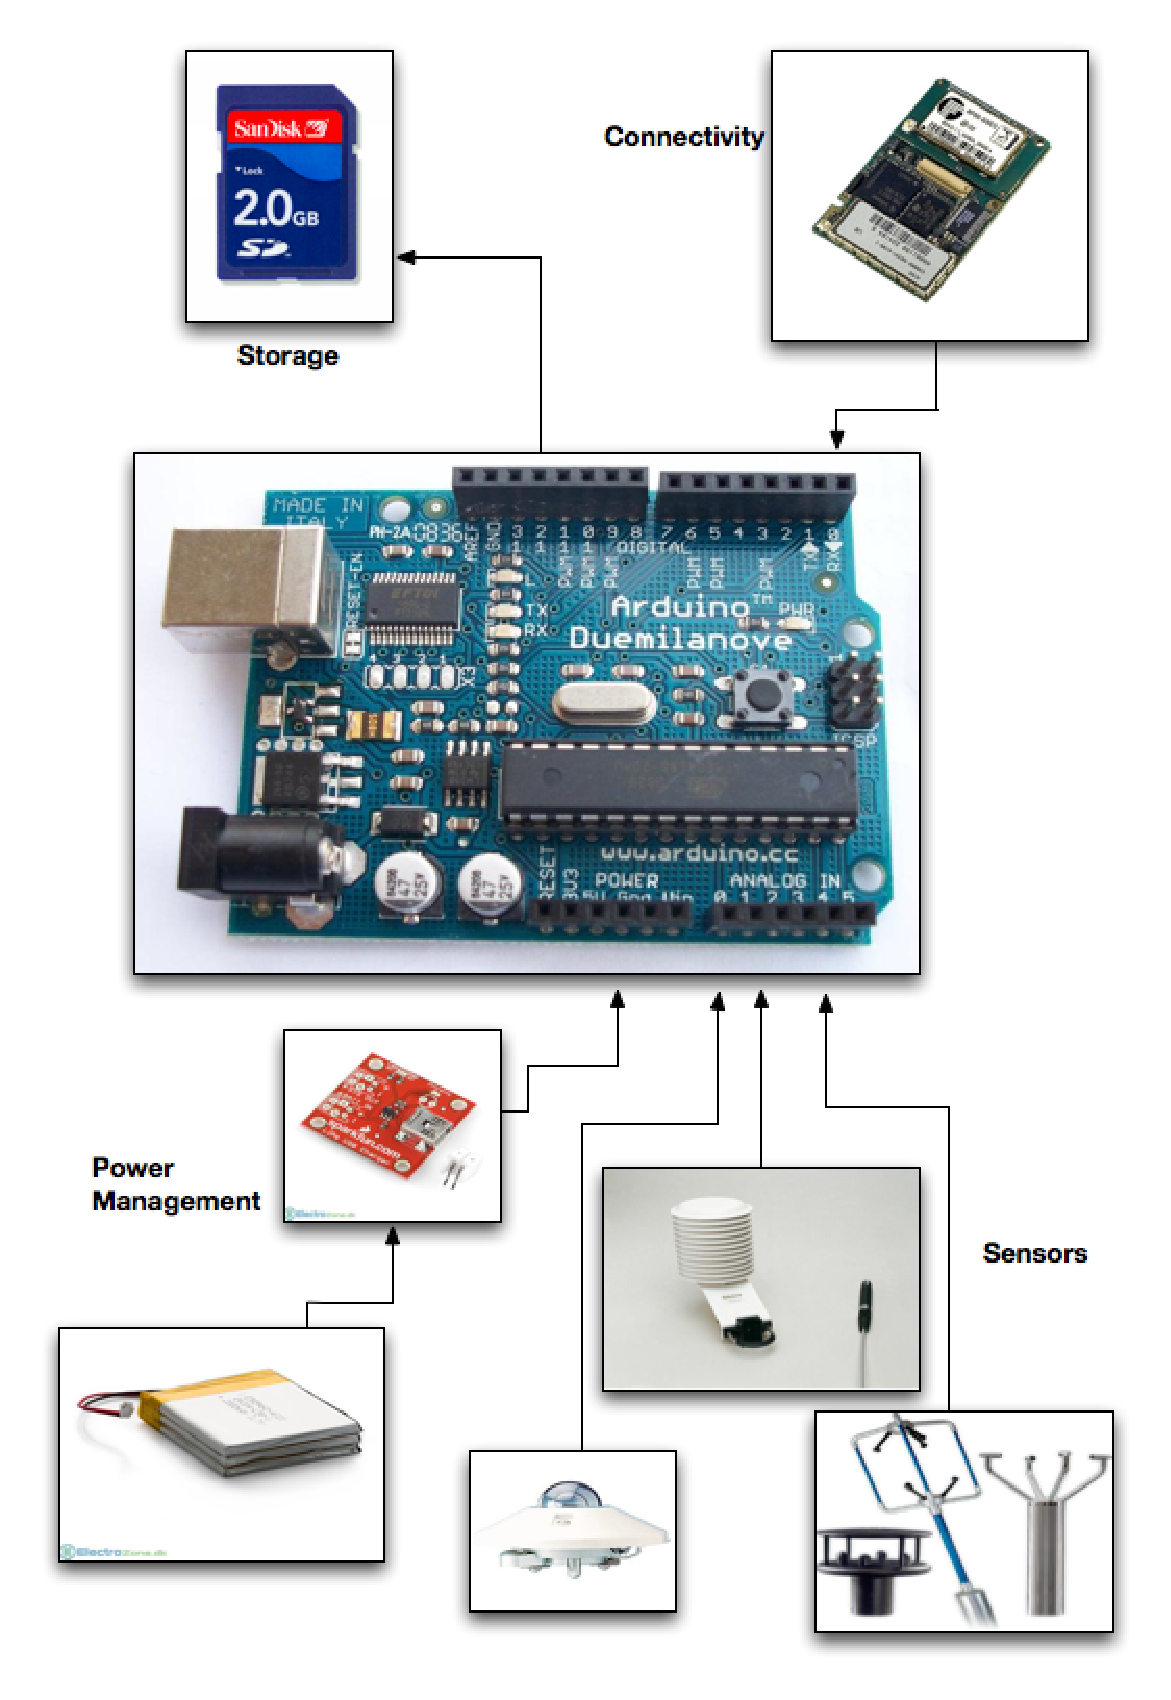
\epsfig{file=figures/overview.eps, scale=0.4}
\caption{Overview of the datalogger}
\label{overview}
\end{figure}
As the simplified figure \ref{overview} shows, the system has 4 components:
\begin{itemize}\addtolength{\itemsep}{-0.5\baselineskip}
\item Storage: SD card
\item Connectivity: GSM/GPRS network
\item Power: Lithium Polymer battery with charger circuit
\item Sensors: Wind vane, Anenometer, Temperature..
\end{itemize}
\subsection{Storage}
For storage, solid state storage is needed, as temperature changes do not go well with moving parts in harddrives. The capacity of modern memory cards are more then sufficient for recording text/binary data for an extended period of time. The simplest cards to interface with a microcontroller are the SD/microSD/MMC cards, as they support the SPI inferface out of the box, which means they can be plugged straight into the microcontroller and used. 
\subsection{Connectivity}
Since the data logger is installed in remote locations, the only two communication options available are the cellural network or a satellite uplink. Since there is cellural coverage in the areas the data logger will be installed, there is no need for the more expensive satellite. 

There are a few complications to consider with providing a communication option for a data logger though. The battery life will be severely affected, as the data transmission consumes a lot of power. There is also an additional cost of an abonnement with the phone company as well as some data charges per MB of transmitted data.  

\subsection{Power}
\begin{figure}[!ht]
\centering
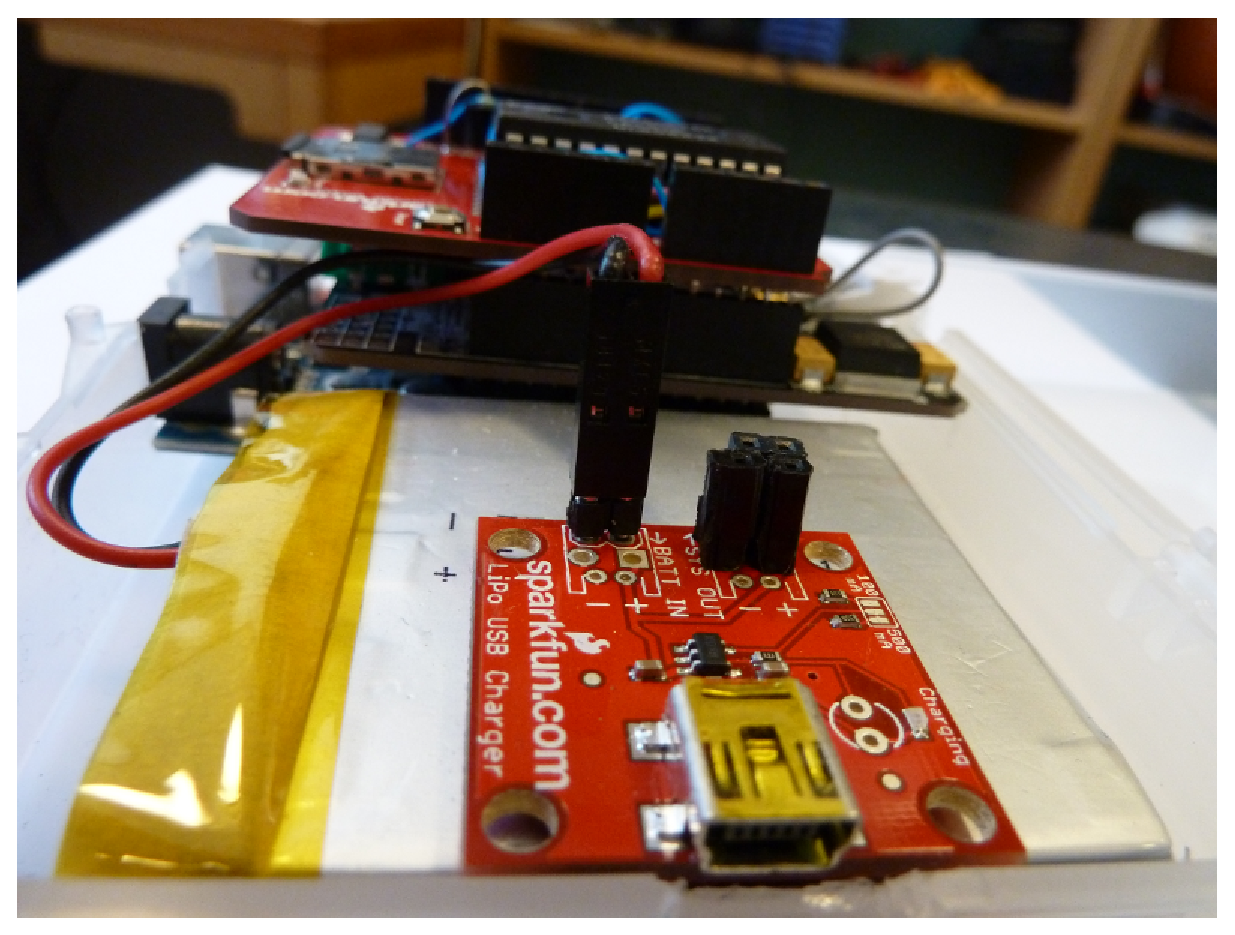
\epsfig{file=figures/battery.eps, scale=0.4}
\caption{The battery for the current prototype}
\label{nanortalik}
\end{figure}

For power, a Lithium Polymer battery was chosen, which is small, lightweight, has a large capacity and can work at low temperatures (efficiency decreases below -25C). 
To charge the battery, a single cell LiPoly charger is used, which can accept 5V up to 500mA, provided by an USB plug. In the places where there will be access to the power grid, an USB charger can be used to trickle charge the battery when there is power, and revert to the battery power when there is a power outage. 
Solar or wind charging should also be possible by regulating the input voltage to the charger.

\subsection{Sensors}
While the sensor choice is not directly related to the datalogger, it is important to be able to interface with all the sensors. So far, 4 different types of signals have been identified:
\begin{itemize}\addtolength{\itemsep}{-0.5\baselineskip}
\item Analog (almost constant) voltage input (temperature sensor, wind vane, humidity, barometric pressure)
\item Analog sine wave input [counter] (anenometer)
\item Digital input (ice sensor, rain gauge)
\item Digital input [counter] (anenometer, rain gauge)
\item Digital output (control signals for equipment)
\end{itemize}
As it can be seen above, these signal types are used by all the equipments, so the data logger has to support them. Fortunately, this can be done relatively easily with modern microcontrollers.

\section{Current progress}
\subsection{The device}
The progress has been relatively good with the project, as the major hardware components have been acquired. On the software front there is still a lot of work to do, but that is only a matter of time. 

The hardware is based on the Arduino Uno/Duemilanove, a Seedruino GSM/GPRS shield, a Sparkfun microSD shield, and a HEF6067BP 16 channel analog multiplexer.
With this, the device is capable of saving data to cheap and readily available microSD cards (up to 4GB currently), send the data by SMS or TCP/IP using the GSM module, have up to 16 analog/digital inputs, and 6 digital outputs for control signals.   

\begin{figure}[!ht]
\centering
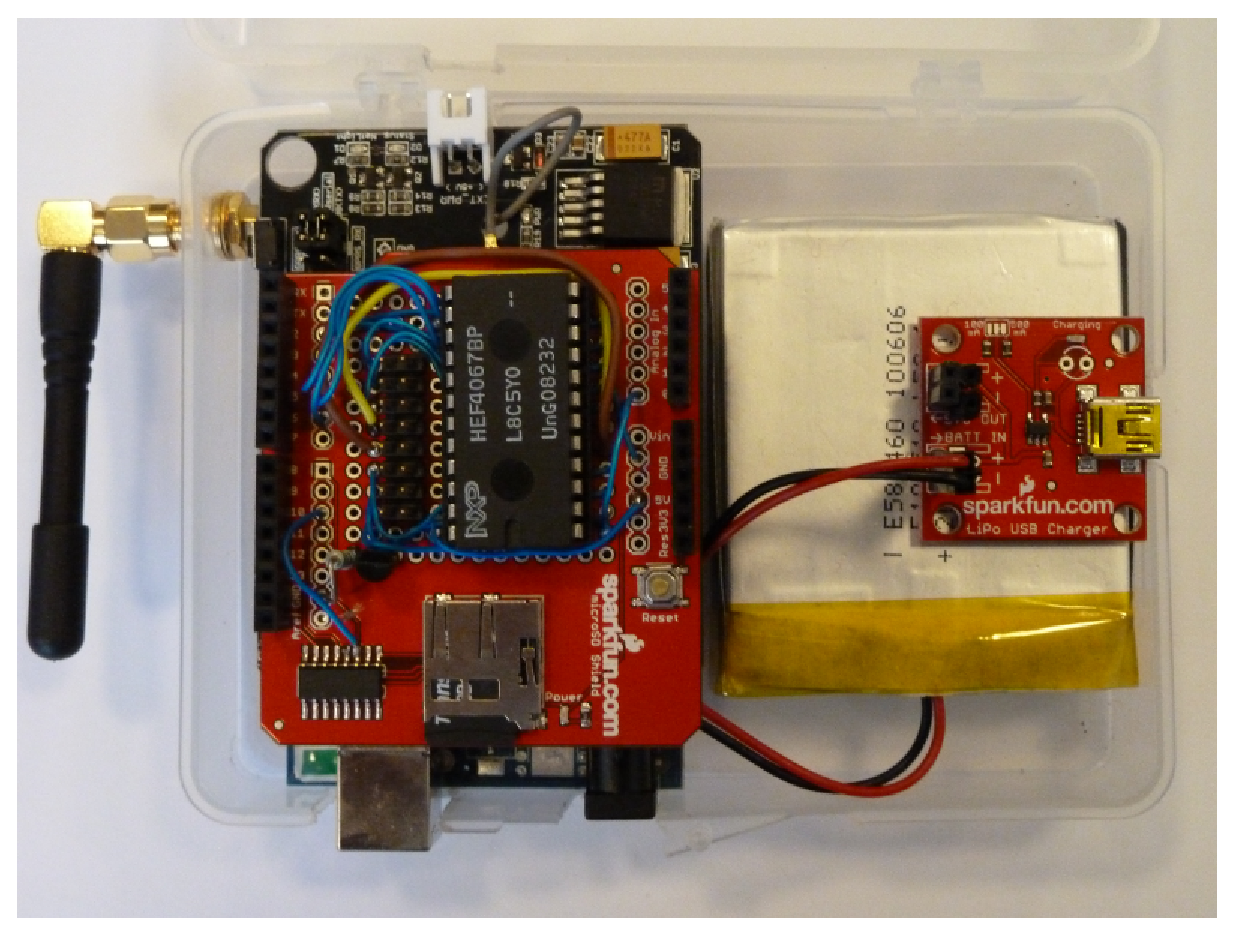
\epsfig{file=figures/topview.eps, scale=0.4}
\caption{Top view of the prototype}
\label{topview}
\end{figure}

\subsection{Testing}
So far the testing on the sensor side has been done using an analog thermometer (KTY81-220), and an analog anenometer (NRG \#40C). These have been hooked up to the 16 channel analog multiplexer, and all the channels have been read out by the microcontroller sequentially. 
The latency for reading out all the 16 channels sequentially has been around 2 ms, which suggests that each channel can be polled at a 500Hz freqency, which should suit most of the applications. If needed, a single channel can be polled at a higher freqency as there is no delay in reading the other channels.

The communications side has been tested too. Phone calls were successfully made, received and terminated using the module, SMS has also been sent and received without any problems. A connection was also successfully made to the GPRS service, allowing TCP/IP communication using the on-board TCP/IP stack of the GSM modem.

The (micro)SD card has also been verified to work with the shield. It can use a FAT32 filesystem, so the card can be pulled out of the module and plugged straight into a computer for copying the data off the card. Based on some performance testing, the write speed to the card was around 80 KB/s while the read speed was 220KB/s, which are both more than sufficient for saving data at a specified interval.
There is a limitation of the currently used SD card library though, it only allows a single open file, which either means that a "system.log" file needs to be opened to save device specific logs, while the data files need to be opened on saving the recorded values.

Some battery testing has also been done, and the system could run for more than a week at full power including the GSM module from the current 6000mAh battery. This is expected to increase by a lot once the hardware watchdog is also enabled, and the GSM module can be switched on and off programatically.

\section{Planning}
While the planning is somewhat dependent on the rest of the equipment and sensors (which are specified by Adriana), there are some known plans which are worth mentioning here.

\subsection{Location}
There are two locations where the logger will be installed, one is Nanortalik and another one is TREF. Both of these locations are in the south of Greenland. (See Figure \ref{southgl})
\begin{figure}[!ht]
\centering
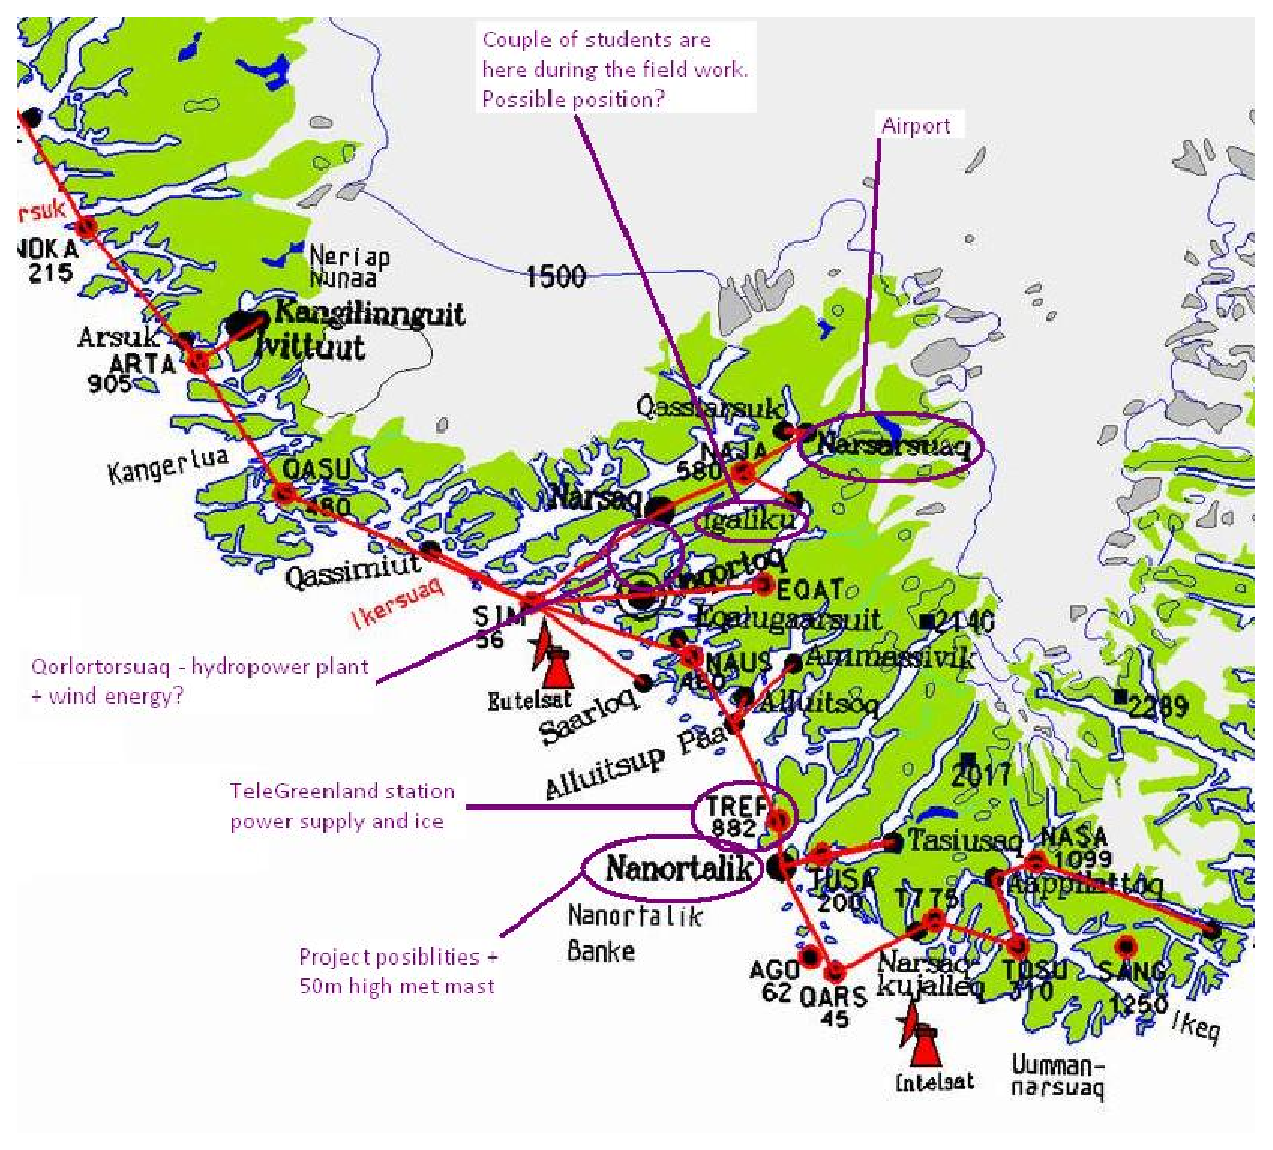
\epsfig{file=figures/southgl1.eps, scale=0.4}
\caption{Map of South Greenland}
\label{southgl}
\end{figure}

\subsection{Nanortalik}
\begin{figure}[!ht]
\centering
\epsfig{file=figures/nanortalik.eps, scale=0.33}
\caption{The red dot indicates where the metmast is in Nanortalik}
\label{nanortalik}
\end{figure}

In Nanortalik, we will be using an existing 50 meter tall metmast to put on additional sensors and the data logger.

\subsection{TREF}
\begin{figure}[!ht]
\centering
\epsfig{file=figures/tref.eps, scale=0.2}
\caption{TREF}
\label{tref}
\end{figure}
TREF is located on top of a mountain close to the ocean, which offers a good spot for measuring icing of different equipment. Here a 3 meter tall metmast will be erected and several sensors placed including the data logger. (Figure \ref{tref})

GPS coordiates: N 60012.923, W 045022.093

\subsection{Schedule}
The schedule so far looks like so:
\begin{itemize}\addtolength{\itemsep}{-0.5\baselineskip}
\item Day 1: Install first data logger in Nanortalik
\item Day 2: Study the power grid/energy systems/factories in Nanortalik
\item Day 3-5: Trip
\item Day 5-12: Install data logger on TREF  
\end{itemize}
This has not been finalized yet, so it is still subject to change.

%\nocite{*}
%\bibliographystyle{abbrv}
%\bibliography{project}  % sigproc.bib is the name of the Bibliography in this case
% You must have a proper ".bib" file
%  and remember to run:
% latex bibtex latex latex
% to resolve all references
%
% ACM needs 'a single self-contained file'!
%
\end{document}
